\subsection{Slučaj upotrebe: Kreiranje zaposlenog i korisničkog naloga}

\subsubsection*{Kratak opis:}

Administrator unosi podatke o novom zaposlenom, dodeljuje mu ulogu i kreira korisnički nalog.

\subsubsection*{Akteri:}
\begin{itemize}
	\item \textbf{Administrator} -- upravlja evidencijom zaposlenih i njihovim nalozima.
\end{itemize}

\subsubsection*{Postuslovi:}
\begin{itemize}
	\item Zaposleni je evidentiran u sistemu, a njegov nalog je kreiran sa privremenom lozinkom.
	\item Sistem je evidentirao promenu.
\end{itemize}

\subsubsection*{Osnovni tok:}
\begin{enumerate}
	\item Administrator bira opciju „Dodaj zaposlenog“.
	\item Sistem prikazuje formu za unos podataka.
	\item Administrator unosi podatke o zaposlenom.
	\item Administrator dodeljuje zaposlenom jednu ili više uloga.
	\item Sistem prikazuje prava koja proističu iz izabranih uloga.
	\item Administrator potvrđuje unos.
	\item Sistem proverava ispravnost podataka i jedinstvenost korisničkog imena i e-mail adrese.
	\item Sistem kreira nalog, generiše korisničko ime i privremenu lozinku i evidentira promenu.
	\item Sistem prikazuje kredencijale Administratoru.
	\item Administrator prosleđuje kredencijale zaposlenom.
\end{enumerate}

\subsubsection*{Podtokovi: /}

\subsubsection*{Alternativni tokovi:}

\paragraph*{A1: Neispravni ili nepotpuni podaci}
\begin{itemize}
	\item Ovaj tok se dešava u koraku 7 ukoliko obavezna polja nisu popunjena ili su u neispravnom formatu.
	\item Sistem prikazuje poruku o grešci i označava neispravna polja.
	\item Povratak na korak 3 osnovnog toka.
\end{itemize}

\paragraph*{A2: Zaposleni već postoji}
\begin{itemize}
	\item Ovaj tok se dešava u koraku 7 ukoliko korisničko ime ili e-mail adresa već postoje u sistemu.
	\item Sistem obaveštava Administratora o duplikatu i prikazuje postojeći zapis.
	\item Ako je u pitanju greška u unosu, Administrator ispravlja podatke i povratak je na korak 3 osnovnog toka.
	\item Ako je zaposleni već evidentiran, slučaj upotrebe se završava neuspešno.
\end{itemize}

\subsubsection*{Specijalni zahtevi: /}

\subsubsection*{Dodatne informacije:}
\begin{itemize}
	\item Polja forme uključuju ime, prezime, e-mail, telefon, datum zaposlenja, radnu poziciju i jednu ili više uloga.
	\item Korisničko ime sistem generiše automatski.
\end{itemize}

\begin{figure}[H]
	\centering
	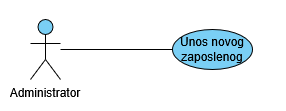
\includegraphics[width=\textwidth]{./dijagrami/dijagrami_slucajeva_upotrebe/slucaj_upotrebe_unos_novog_zaposlenog.png} 
	\caption{Dijagram slučaja upotrebe ,,Kreiranje zaposlenog i korisničkog naloga''}
\end{figure}

\begin{figure}[H]
	\centering
	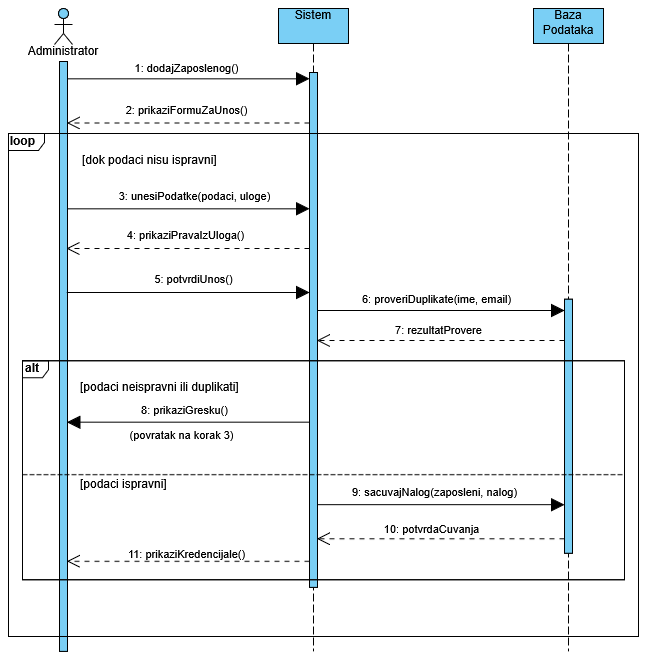
\includegraphics[width=\textwidth]{./dijagrami/dijagrami_sekvence/kreiranje_naloga.png} 
	\caption{Dijagram sekvence ,,Kreiranje zaposlenog i korisničkog naloga''}
\end{figure}

\newpage